\documentclass[11pt,a4paper]{article}
\usepackage{tikz}
\usetikzlibrary{arrows.meta,positioning}
\usepackage{tabularx}
\usepackage{amsmath,amssymb,amsthm}
\usepackage{geometry}
\geometry{margin=1in}
\usepackage{hyperref}
\usepackage{graphicx}
\usepackage{setspace}
\onehalfspacing

\title{\textbf{Paper G-03: AI Emergence:\\ A Constraint-Driven Flux Dynamics (CDFD) Perspective}}
\author{Steve Bico Mujjabi, MD\\
\small Independent Researcher\\
\small Founder, Vura Labs\\
\small Kampala, Uganda\\
\small ORCID: 0009-0001-0556-5516}
\date{August 2026}

\begin{document}
\maketitle

% BEGIN SHARED-METHODS POINTER
\noindent\textit{Shared Part IV notation and evidence boundaries are defined in \path{PART_IV_METHODS_AND_CLAIM_BOUNDARY.md}. This paper states only its local observables, comparison, and failure conditions.}
% END SHARED-METHODS POINTER


\begin{abstract}
This paper develops a falsifiable CDFD/AFL model of AI Emergence. It maps data, compute, models, feedback, deployment demand, and social attention to driving flux $\Phi$, compute, data quality, governance, evaluation, energy, and oversight to active constraint $C$, learning, tool use, modularity, monitoring, correction, and institutional response to responsiveness $S$, and weights, deployed systems, standards, incidents, incentives, and feedback history to structural memory $M_s$. The target outcome is capability, reliability, diffusion, risk, and social adaptation, tested against scaling records, evaluations, deployment telemetry, incidents, policy changes, and energy use. The paper treats universality as a shared model architecture rather than an assertion that unlike systems have the same material mechanism. It states the negative result that would make the mapping unnecessary and places the domain claim inside the cumulative CDFD programme and its reproducible runtime boundary.
\end{abstract}

\section{Introduction}

Artificial neural networks simulate learning by iteratively adjusting millions or billions of parameters to minimize a loss function against a training dataset. The current paradigm of AI development relies on massive brute-force scaling: pumping enormous volumes of data through immense clusters of GPUs.

While this has yielded emergent cognitive behaviors, the trajectory is fundamentally thermodynamic. The network is essentially an active engine consuming information and energy to produce structured mathematical memory. In CDFD terms, a deep learning model is an adaptive topological surface attempting to balance immense throughput against strict physical and architectural bottlenecks.

\section{Neural Architecture as an Adaptive Surface}
We map the training of a neural network to the CDFD life number equation:
\begin{equation}
    \Psi_s = \left( \frac{\Phi}{C} \right) \cdot S \cdot M_s
\end{equation}

In an artificial intelligence system:
\begin{itemize}
    \item \textbf{Flux ($\Phi$)}: The gradient updates and the raw throughput of training tokens (data flow).
    \item \textbf{Constraint ($C$)}: The rigid, fixed architecture of the network (e.g., fixed number of layers and attention heads), as well as the physical hardware limits (memory bandwidth and thermal dissipation).
    \item \textbf{Responsiveness ($S$)}: The available parameter space (model width and depth) that can actively adapt to the incoming gradients.
    \item \textbf{Memory ($M_s$)}: The accumulated, frozen weights of the network. As the model trains, it transitions from a high-entropy chaotic state into a low-entropy locked state (overfitting or saturation).
\end{itemize}

\subsection{The Saturation Threshold and Catastrophic Forgetting}
During early training, $S$ is high (many free parameters) and $M_s$ is low. The network efficiently absorbs the flux $\Phi$. $\Psi_s \approx 1$.

However, as training progresses, the weights solidify into fixed representations. The systemic memory $M_s$ increases, locking the topology. If new, out-of-distribution data ($\Phi$) is introduced, the fixed architectural constraints ($C$) cannot flex to accommodate it. The network enters an over-constrained regime ($\Psi_s \ll 1$). To learn the new data, it must overwrite its existing weights, destroying its previous capabilities---a phenomenon known in machine learning as "catastrophic forgetting."

Unlike biological brains, which dynamically grow new synapses and prune old ones (active restructuring of $C$ and $S$), current LLMs have fixed, static constraints.

\section{The Path to General Intelligence}
The CDFD framework models the condition that that you cannot achieve infinite adaptability in a system with fixed static constraints. If $C$ is locked, $\Psi_s$ will enter an overload regime as $M_s$ saturates.

True Artificial General Intelligence (AGI) requires an architecture where the constraint $C$ itself is a dynamic variable governed by the differential equation $\frac{\partial C}{\partial t} = \alpha |\Phi| - \beta C$. The network must be able to physically or logically grow new architectural branches (neurogenesis) and prune useless nodes to continually maintain $\Psi_s \approx 1$. Liquid neural networks and sparsely activated mixture-of-experts (MoE) are primitive steps toward this, but an AGI must be a fully self-regulating CDFD surface.



\section{Measurement Layer}

% BEGIN PART IV MAJOR CROSS-DOMAIN UPGRADE
\section{Cross-Domain Model Upgrade: Mechanism, Scale, and Tests}

\subsection{Observable Translation}

The paper-specific translation begins with an observable chain rather than a
verbal analogy. For AI Emergence, the proposed drive is data, compute, models, feedback, deployment demand, and social attention.
The active limitation is compute, data quality, governance, evaluation, energy, and oversight. Responsiveness is carried by
learning, tool use, modularity, monitoring, correction, and institutional response, while retained state is represented by
weights, deployed systems, standards, incidents, incentives, and feedback history. The outcome to explain is capability, reliability, diffusion, risk, and social adaptation.

\begin{table}[htbp]
\centering
\small
\caption{Operational CDFD/AFL map for Paper G-03.}
\begin{tabularx}{\textwidth}{|l|X|X|}
\hline
\textbf{Term} & \textbf{Paper-specific observable meaning} & \textbf{Measurement question} \\
\hline
$\Phi$ & data, compute, models, feedback, deployment demand, and social attention & What rate, load, gradient, or demand enters the focal system? \\
\hline
$C$ & compute, data quality, governance, evaluation, energy, and oversight & Which measured bottleneck limits transfer, function, or recovery? \\
\hline
$S$ & learning, tool use, modularity, monitoring, correction, and institutional response & Which process changes effective capacity or reroutes the load? \\
\hline
$M_s$ & weights, deployed systems, standards, incidents, incentives, and feedback history & Which retained state makes equal present loads produce different futures? \\
\hline
$Y$ & capability, reliability, diffusion, risk, and social adaptation & Which outcome is predicted out of sample, with uncertainty? \\
\hline
\end{tabularx}
\end{table}

\begin{figure}[htbp]
\centering
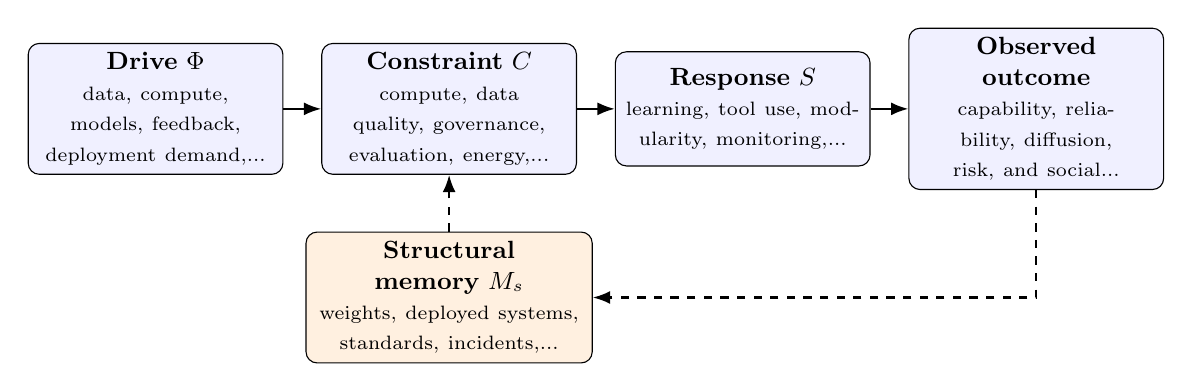
\begin{tikzpicture}[
    node distance=0.48cm,
    every node/.style={font=\small},
    box/.style={draw, rounded corners, align=center, minimum height=1.45cm, text width=3.0cm, fill=blue!6},
    memory/.style={draw, rounded corners, align=center, minimum height=1.25cm, text width=3.4cm, fill=orange!12},
    flow/.style={-{Latex[length=2.2mm]}, thick},
    feedback/.style={-{Latex[length=2.2mm]}, thick, dashed}
]
\node[box] (drive) {\textbf{Drive $\Phi$}\\\scriptsize data, compute, models, feedback, deployment demand,...};
\node[box, right=of drive] (constraint) {\textbf{Constraint $C$}\\\scriptsize compute, data quality, governance, evaluation, energy,...};
\node[box, right=of constraint] (response) {\textbf{Response $S$}\\\scriptsize learning, tool use, modularity, monitoring,...};
\node[box, right=of response] (outcome) {\textbf{Observed outcome}\\\scriptsize capability, reliability, diffusion, risk, and social...};
\node[memory, below=0.72cm of constraint] (memory) {\textbf{Structural memory $M_s$}\\\scriptsize weights, deployed systems, standards, incidents,...};
\draw[flow] (drive) -- (constraint);
\draw[flow] (constraint) -- (response);
\draw[flow] (response) -- (outcome);
\draw[feedback] (outcome.south) |- (memory.east);
\draw[feedback] (memory.north) -- (constraint.south);
\end{tikzpicture}
\caption{Paper G-03 observable CDFD/AFL architecture for AI Emergence. Solid arrows give the proposed forward chain; dashed arrows make history-dependent feedback explicit.}
\label{fig:g03-architecture}
\end{figure}

\subsection{Paper-Specific Causal Hypothesis}

For this paper, the hypothesized causal sequence is specific. A change in
data, compute, models, feedback, deployment demand, and social attention arrives faster than learning, tool use, modularity, monitoring, correction, and institutional response can compensate.
This raises or redistributes compute, data quality, governance, evaluation, energy, and oversight. If the load persists,
the retained state encoded by weights, deployed systems, standards, incidents, incentives, and feedback history changes the next response, so a later event of equal
magnitude can produce a different trajectory in capability, reliability, diffusion, risk, and social adaptation. The
scientific task is to estimate that sequence against the best ordinary model of
the domain, not merely to redescribe the outcome after it occurs.

\subsection{Cross-Scale Translation Without Mechanistic Erasure}

For the abstract and cognitive systems family, the cross-domain translation compares information-bearing activity, limited channels or institutions, adaptive reorganization, and retained semantic or technical structure. Because meanings and goals are not conserved physical quantities, every mapping must state its observational unit and avoid treating metaphor as measurement. \cite{Shannon1948,BarabasiAlbert1999,WattsStrogatz1998,Turing1952,BakTangWiesenfeld1987}
The required scale declaration for this paper is microseconds to decades; model components to socio-technical ecosystems. At short
scales, the key question is whether the incoming drive is transmitted,
buffered, or diverted. At intermediate scales, response changes effective
capacity and network exposure. At long scales, retained structure can alter the
state space itself. A result is genuinely cross-scale only when the aggregation
rule is stated and the same conclusion is not an artifact of averaging.

\subsection{Evidence Ladder and Discriminating Tests}

\begin{table}[htbp]
\centering
\small
\caption{Evidence ladder for Paper G-03. Each rung can fail independently.}
\begin{tabularx}{\textwidth}{|p{0.17\textwidth}|X|X|}
\hline
\textbf{Test} & \textbf{Design} & \textbf{Discriminating result} \\
\hline
Proxy audit & Measure scaling records, evaluations, deployment telemetry, incidents, policy changes, and energy use and preregister how each record maps to $\Phi$, $C$, $S$, $M_s$, and $Y$. & The mapping fails if proxies are non-identifiable, circular, or change meaning across cases. \\
\hline
Load ramp & Apply or observe a capability or deployment shock under contrasting oversight histories while estimating the dominant constraint and response time. & A threshold claim requires a reproducible nonlinear change and uncertainty bounds, not a visually chosen breakpoint. \\
\hline
Recovery and memory & Match present load across units with different histories, then compare recovery paths. & The memory claim requires history-dependent divergence after current conditions are controlled. \\
\hline
Model comparison & Compare the baseline domain model with and without the CDFD/AFL state variables using held-out data. & The paper's stated falsifier is: CDFD variables do not improve capability, failure, or governance-response prediction. \\
\hline
\end{tabularx}
\end{table}

\subsection{Research Programme and Boundary Conditions}

The immediate research programme has four steps. First, construct a documented
dataset from scaling records, evaluations, deployment telemetry, incidents, policy changes, and energy use and retain raw units before normalization.
Second, fit a baseline domain model and report its calibration and out-of-sample
error. Third, add the smallest identifiable CDFD/AFL state extension and test
whether it improves prediction of capability, reliability, diffusion, risk, and social adaptation. Fourth, repeat the
analysis across the declared scale range and publish negative cases as part of
the cross-domain translation audit.

% END PART IV MAJOR CROSS-DOMAIN UPGRADE

\section{Conclusion}
Artificial-intelligence systems face measurable limits in compute, data, energy, evaluation, and governance. CDFD offers a candidate architecture for testing how those constraints interact with learning and deployment history; it does not establish a universal ceiling or guarantee open-ended cognition.
\section*{Conflict of Interest} The author declares no conflict of interest.
\section*{Data Availability}
Part-specific runtime diagnostics are under each Part's \path{outputs/} directory.

Release-wide code: \path{Part_E_Synthesis/supplementary/}.

Generated summaries: \path{Part_E_Synthesis/outputs/}.

Figures: \path{Part_E_Synthesis/figures/}.


\section{Reference Layer}
\bibliographystyle{plain}
\bibliography{universal_afl_references}
\end{document}
